\documentclass[12pt,a4paper]{report}

\usepackage[cm]{fullpage}
\usepackage{paralist}
\usepackage{graphicx}
\usepackage{wrapfig}

\title{Workflow thing}

\author{Michiel Johan Baird \\
        Department of Computer Science \\
        University of Cape Town
        \thanks{Funded by NRF}
    \\   \small{Supervisor: Dr. Hussein Suleman} }

\begin{document}
\maketitle
\newpage
\tableofcontents
\newpage
\listoffigures
\newpage
\chapter{Introduction}
\chapter{Background}
\chapter{Design}
\section{Introduction}
In order to answer the research question, the design of the system needs
to take the in the considerations of the client. The  system
was implemented in three design iterations. These iterations are
as follows: \begin{inparaenum}[(i)] \item Feasability design;
\item Workflow system design; and \item User Interface design.
\end{inparaenum} The methodology used is to design, implement
and evaluate the system at each interations. The evaluation at
each step is then used as additional consideration at the following
design step. This is illustrated by Figure~\ref{design_figure}.

\begin{figure}[!h]
\begin{center}
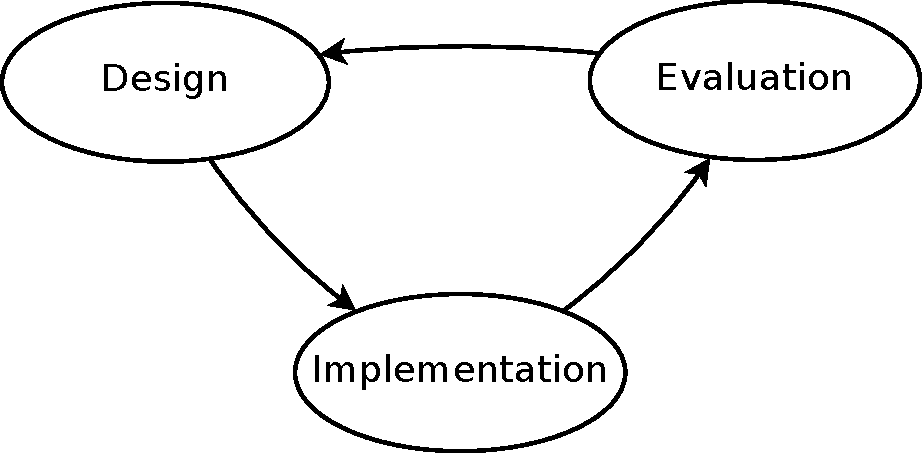
\includegraphics[scale=0.5]{figures/design_cycle.pdf}
\end{center}
\caption{Design Process}
\label{design_figure}
\end{figure}

\noindent This chapter describes the design process followed in the building
of the workflow system. Section~\ref{design_consdierations} describes
the items taken into consideration in the initial design. This is then
followed by process followed during the first iteration in Section~\ref{feasibility}.
Section~\ref{iteration2} follows the design and implementation of the
first functional product, this product is then evaluatated and continues
on the next iteration. Section~\ref{iteration3} follows the critisisms that
were highlighted in the evaluation in Section~\ref{iteration2} and makes
improvements on the design where certain functionality can


\section{Design Considerations\label{design_consdierations}}
This system is developed for the Zamani Project. This requires
a thorough understanding of the requirements that exist within
the team. This then has to be combined with the general requirements
of a workflow system.
\begin{description}
    \item[Workstation configuration] \hfill \\
        Within the Zamani team each member has a workstation on campus.
        These workstations vary in specification but are all locally
        connected to a highspeed local network. These workstations are
        predominantly \emph{Microsoft Windows 7} based machines.  On this
        network there is also as server present. This server is used as
        a repository for the sites. Figure~\ref{network_setup} shows the setup
        of the workstations. Files required to process any particular task is
        typically transferred using the network or via removable drives.
\begin{figure}[!h]
    \begin{center}
        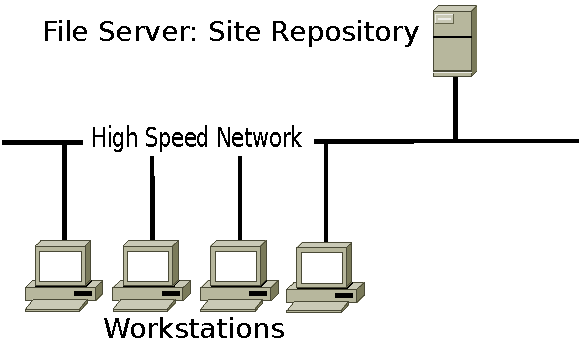
\includegraphics[scale=0.6]{figures/networklayout.pdf}
    \end{center}
    \caption{Zamani Network Configuration}
    \label{network_setup}
\end{figure}
    \item[Task Variety] \hfill \\
        The team's main tasks involve creating derivative data off of laser
        scans, photo graphs and other source data. A large portion of these
        tasks can be automated, whilst others require manual processing by the
        team. As such the tasks can be divided into two types. User tasks and
        server tasks.


    \item[Dataflow model] \hfill \\
        The process involves the data constantly moving between the server
        and workstations with data elements being added at every step. These
        flows are rather complex and relate closely to th workflow of the
        project.  Given the scale of the data being processed, transferring the data
        from one end to another has a large cost. As such this cost should
        be factored into the design.


    \item[Staff Turnover] \hfill \\
        The project consists of a core number of individuals as well as
        a group of interns that cycle in and out of the project on a regular
        basis. This would have an impact at the task
        level if a user fails to complete a particular task before leaving
        the project. Due to the high staff turnover rate this would
        be a frequent occurrence and as such would have to be sufficiently
        dealt with by the system.

    \item[Repeatability] \hfill \\
        In creating this data the same processes are essentially followed
        on all sites. In the design of the processes these would need to
        be reusable on different sites with very little effort. This
        will aid in the easy repeatability of the science.

    \item[Integration with existing software] \hfill \\
        The Zamani project uses a wide variety of programs is used during
        the processing of this data. The workflow system would as such
        would have to integrate with this software as well.

    \item[System Backup] \hfill \\
        Each site consists out of a set data items. This data is very valuable
        and is often times irreplaceable. In the case of a system failure
        the loss of the data would have great costs. As this system would
        be controlling these items it would have to allow for the site
        to be backed up.

    \item[Provenance] \hfill \\
        Provenance refers to the documented history of an object\cite{moreau2008open}. For
        digital objects this refers to all the objects, processes and agents
        involved in the life cycle of the object. Provenance is perceived as
        a crucial component in workflow systems. This is designed to aid in
        analysis of systems and help ensure reproducibility. The Open
        Provenance Model was designed represent the capabilities of a system.
        This allows the technology to be defined in an agnostic way and
        allows systems such as this to be built that uses this model.

        This model consists of three primary entities: \begin{inparaenum}[(i)]
        \item Artifacts; \item Process; and \item Agents.\end{inparaenum} These
        artifacts are joined using relations and dependencies.
        Figure~\ref{provenance}  shows the relations between the entities of
        the model. The benefit of using such a model is that it has been
        extensively tested in other similar systems with great success.
        \begin{figure}[!hb]
            \begin{center}
                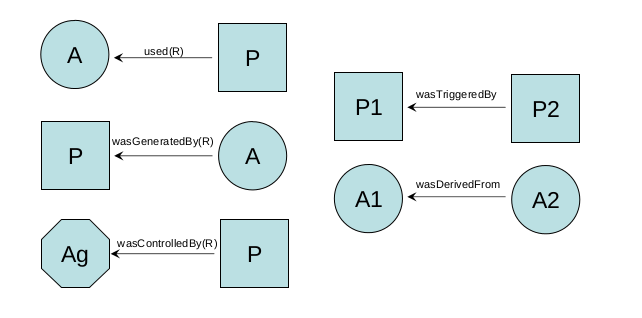
\includegraphics[scale=0.5]{figures/provenance_edges.png}
            \end{center}
            \caption{Edges in the provenance model}
            \label{provenance}
        \end{figure}
\end{description}

\section{Feasibility Demonstration\label{feasibility}}

The core focus of the this iteration to ensure that the core types of tasks
in the system would be supported. The main tasks being, user-tasks and tasks
that can be automated. During this portion a significant amount of time and
effort was spent on comparing different systems with each other.

This phase produced a small system, that supported very primitive manual and automatic
tasks. The system was integrated with \emph{Kepler}~\footnote{
The Kepler Project: www.kepler-project.org }, and could copy over files to a remote
host. The tasks could be signaled as being, ``Not Done'', ``In Progress'' and ``Complete''.


\subsection{Design}
The initial design focussed on enabling the type of tasks required by the system.
These tasks can be abstracted into two main types: \begin{inparaenum}[(i)] \item
Manual User Tasks; and \item Automated tasks\end{inparaenum}.


The workflow-management system will be run on the same server that hosts the central
site repository. This would allow inherent data locality therefore would allow for
efficient server operations on the data. These operations would be performed on data
of a given site. Sites can be abstracted to a large hierarchical collection of data
items. To aid in the repeatability of the system the hierarchy of each of these
sites should kept consistent both within the main repository and on the user hosts.

\subsubsection*{Server Task}
The first type of task that would need to be facilitated by the system are those
tasks that can be done automatically by the system and requires no interaction
from a user. These include removing duplicate points in input data, or changing
a file to a particular format. To avoid the high cost of transferring data these
tasks are performed on the server itself.

\subsubsection*{User Task}
The second type of task that needs to facilitated within the system is manual
tasks performed by the members of the team. During such a task particular data
elements of the site are required to create new derived data elements. As all the
team members cannot work on the server, the required files would need to be moved
to the respective workstations that. Figure~\ref{data_flow} shows the data flow for any given
User task.
\begin{figure}[!h]
    \begin{center}
        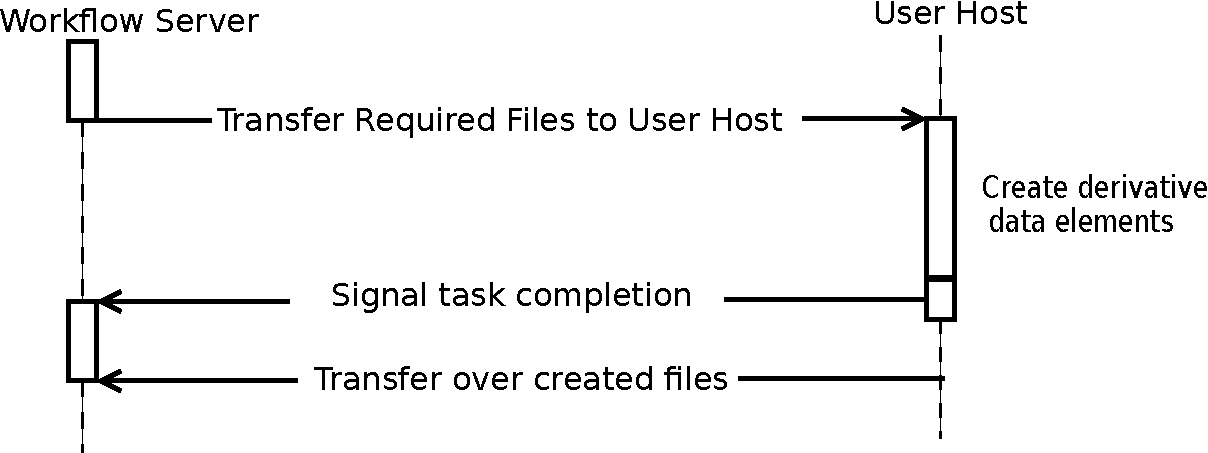
\includegraphics[scale=0.5]{figures/data_flow.pdf}
    \end{center}
    \caption{Data flow in user task}
    \label{data_flow}
\end{figure}

\subsubsection*{Basic Task Model}
These task types can be abstracted for the workflow system into a general
task type. This allows the system to handle them indiscriminately. The basic
requirements of a task is to take a set on input data and produce a set
of output data, these are mapped to artifacts in the provenance model.
This will allow the tasks to be chained together to form
a complex workflow. This task maps to the \emph{Process} entity in in the
provenance model. Each task would be assigned to a assigned to a user, which
maps to an agent in the provenance model.

\subsubsection*{Kepler integration}
Kepler is a popular workflow system, with plenty of pre-built models to
facilitate complicated workflows. Ideally the system would need to be able
to integrate with Kepler so that it can harness the existing capability
of the system.

\subsubsection*{Site Layout}
Within the Zamani Project the data is organised at the root level in terms of
the physical site to which the data corresponds. Since the goal is to have the
tasks be executed on a variety of different workstations, the data management
would be greatly simplified if the folder structure is the same on the workstations
and the server. For this reason workstations and the workstations will have a
an identical directory structure with the site being regarded as the root. This
layout could be changed from site to site to allow for more flexibility.

\subsection{Implementation}

The first round of implementation set out to test the feasibility of the
core components required within the system. As shown above this is identified
as setting up a the framework for the User and Server Tasks. This was done using
Kepler, Java, and a series of command line tools. This was split into the following
components: \begin{inparaenum}[(i)] \item Database; \item Kepler Task Model;
\item and a Kepler File Copier. \end{inparaenum} These could then be packaged
to create complicated workflows that could represent a site.
Figure~\ref{iter1_overview} shows how these components interact with each
other to form the core components of the workflow system.

\begin{figure}[!h]
    \begin{center}
        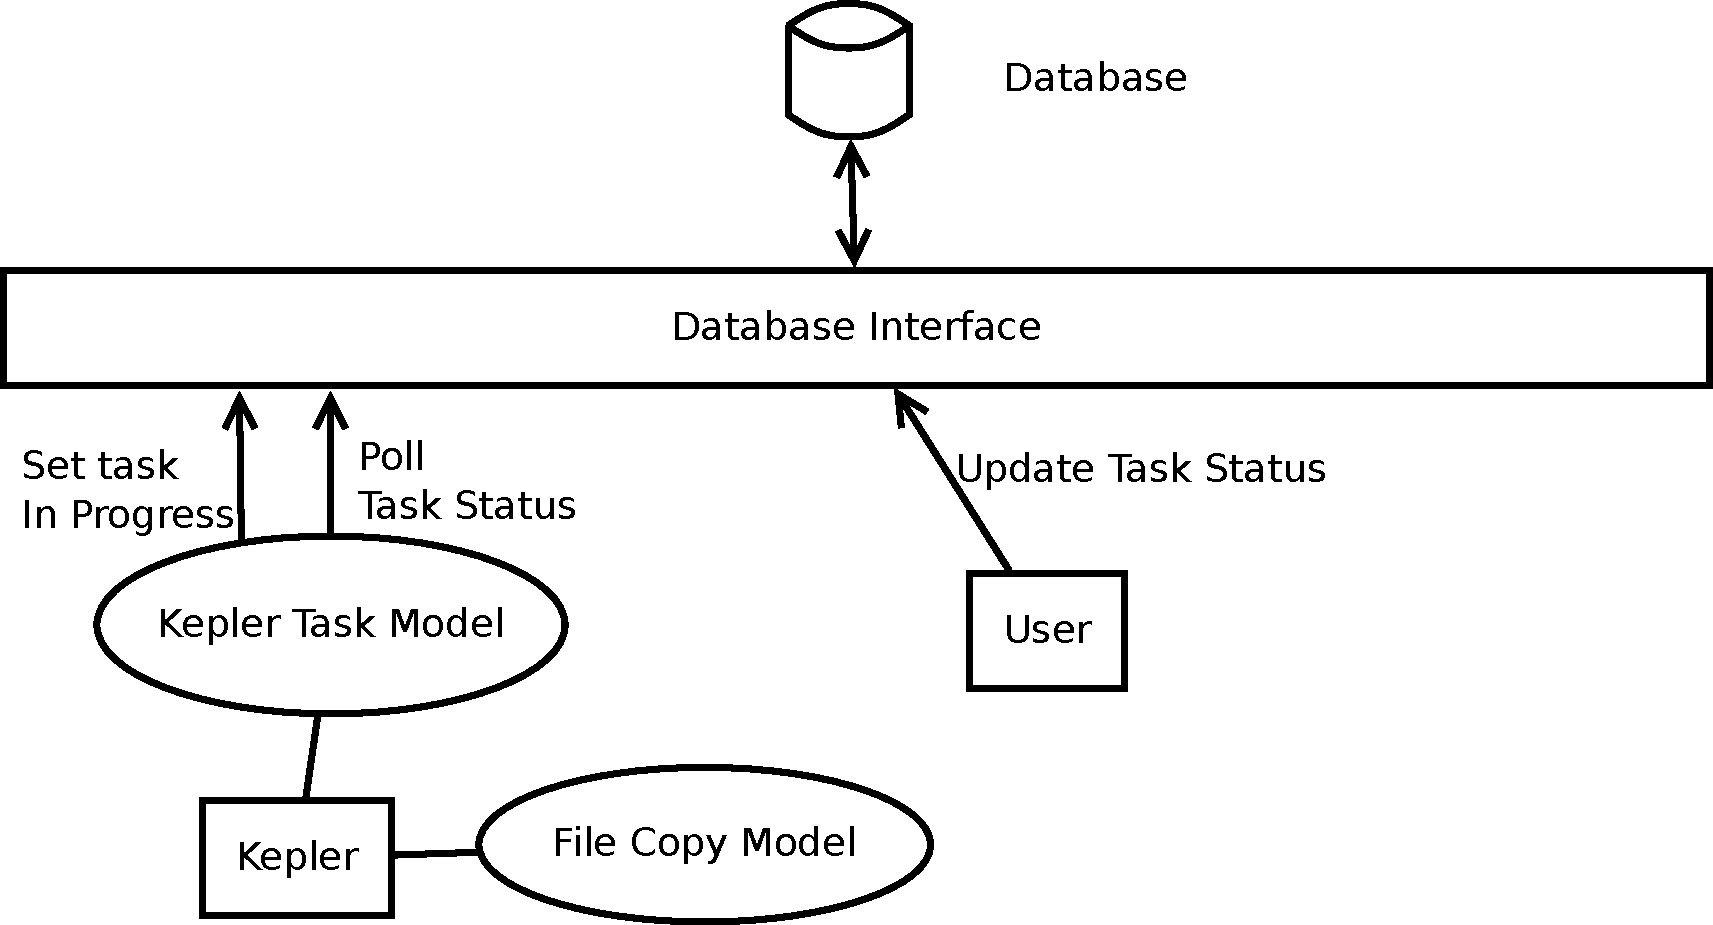
\includegraphics[scale=0.35]{figures/iter1_impl.pdf}
    \end{center}
    \caption{Feasibility components}
    \label{iter1_overview}
\end{figure}

\subsubsection{Database}
In order to keep track of the tasks a MySQL database was used. Tasks could be added
to the database along with a status. As a task progressed thorough the process its
status would be updated which would trigger events in the system. Initially tasks would
have three valid statuses: ``NOT DONE'', ``IN PROGRESS'' and ``DONE''. The database would
be updated by small scripts that could be called by Kepler.

\subsubsection{Kepler Task Model}

This model is used to launch user tasks. The model then polls the database for
status changes of the task. As soon as a user then completes the task the
database is updated, the model would pick this up and continue with the process.
Figure~\ref{kepler_task_model} shows the workflow in Kepler for the task model.

\begin{figure}[!h]
    \begin{center}
        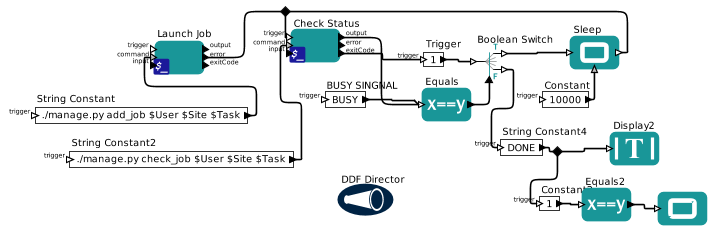
\includegraphics[scale=0.6]{figures/task_model_kepler.png}
    \end{center}
    \caption{Kepler model that launches a user task}
    \label{kepler_task_model}
\end{figure}

Kepler is not ideally suited for user-task as it's primary focus is complex
automation as such support user tasks. It is also highly suboptimal as it needs
continuously poll to determine the status of a given task.

\subsubsection{Kepler File Copier}
User tasks also need files to be copied to the user workstations. For this
a Kepler workflow was built that copies files. Each task has a list with the
files required to complete the task. The model uses SCP to copy over files
to the respective user. Figure~\ref{kepler_file_model} shows how the model
is built in Kepler.

\begin{figure}[!h]
    \begin{center}
        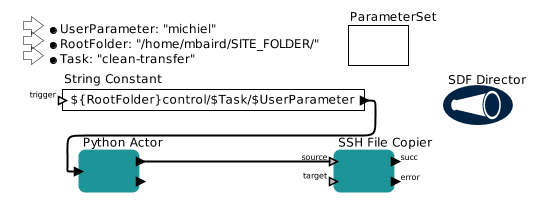
\includegraphics[scale=0.6]{figures/kepler_file.png}
    \end{center}
    \caption{Kepler model that copies files to workstations}
    \label{kepler_file_model}
\end{figure}


\subsection{Evaluation}
Due to the lack of functionality of the first prototype the first
phase of evaluation was rather short. This prototype was demoed to
the second reader (Dr. Bagula). The prototype showed that the core
requirements could be implemented and was critical to develop a more
complete understanding of the problem.


\subsubsection{Dropping Kepler}
Kepler is rather bulky and the user task model is ill suited to the system.
The Zamani Project's tasks fit better to an operational model, whereas Kepler
is suited to more scientific data processing model.

Kepler also does not integrate very well from an interface point of view.
As such it was decided that Kepler would not be used in the next iteration. This
requires that the functionality be replicated in the next iteration.

\section{Functional Design\label{iteration2}}
This section follows the second design iteration using the the first iteration
as a base. The goal of this iteration is to create a workflow system that is
functionally adequite to support the automisation of the workflow for the Zamani
Project.

\subsection{Design}
The design of the second iteration follows a more rigourous process and has the
primary goal of supporting most of the required functionality. The system should
be support multiple users each being able to execute a portion of the workflow
assigned to them.
\subsubsection{Web Interface}
Using a web interface is well suited to the problem. This will allow multiple
users to log in, track and manage their tasks. This could also be hosted on the
same server that would host the primary site repository. Preference and prior
experience experience led to the adoption of Django~\footnote{Django Web Framework
www.djangoproject.com} for this purpose. Django is a Python framework that allows
for rapid web application development. Due to the sort iteration cycles Django is
well suited to be used as the supporting framework for the system.
\subsubsection{Replication of Kepler functionality}
The feasibilty demonstation showed that Kepler has poor support for the user
tasks required within the workflow system. This functionality will need to
be replicated within the new framework. This requires classification of
of the Zamani workflow such that it can be correctly implemented.
A workflow management system can be classified by four different elements
\cite{yu2005taxonomy}:
\begin{description}
    \item[Workflow Design] \hfill \\
        The tasks required within the project are well defined
        data is transformed in a linear manner. Data items do not get iterated over
        once they are complete. Therefore the system would fit a user defined,
        directed acyclic graph. This workflow would be designed my the user to
        allow for arbitruary dependencies.
    \item[Workflow Scheduling] \hfill \\
        Based on the way that the project is currenly executing tasks the scheduling
        would need to need to happen Dynamically with a priority to to determine the
        urgency of any particular task.
    \item[Fault Tolerance] \hfill \\
        Since the system would be dealing with a large amount of data a lot of which
        will be generated by the users themselves, the likelihood that tasks may fail
        is quite high. Therefore it needs to be mediated. Since the workflow models
        would be manually created by a user workflow level errors will not be taken
        into account. The system will however have to be able to deal with task level
        failures. The mediation process would include: the ability to retry a task
        and modify the node on failure. Both of these would have to be mediated manually
        by the user.
    \item[Data Movement] \hfill \\
        New data is is continuosly generated and as such the movement of the data needs
        to be controlled, the goal is to automate the data movement, using a centralised
        repository that maintains the authority on data.
\end{description}
Django is built using Python and uses a \emph{Model View Controller}
architecture\cite{leff2001web}. This model seperates the system into three parts: the
data, the control logic and the presentation of the data. The MVC framework would allow for
the workflow logic to be built and executed independently of the User representation of it.

\subsubsection{Particpatory Design Session}

To ensure that the product meets the needs of client they were made active participants
in the design process. The methodology used during this is Participatory design
\cite{muller1993participatory}. Due to limited time this is selectively applied. The
team of four was brought together for PICTIVE session \cite{muller1991pictive}.
The method used can be outlined as follows:
\begin{inparaenum}[(i)]
\item General Requirements gathering;
\item defining the task flows; and
\item a graphical user interface PICTIVE design session.
\end{inparaenum}

The session identifified the core tasks that need to be supported. These
include the following:
\begin{itemize}
    \item Worflow Setup
    \item Template Functionality
    \item Progress Inidicators
    \item Task time information
    \item Task control from a user perspective
    \item Logging Functionality
\end{itemize}
These tasks were then further developed to create a logical usecase. The
most important functionality was define within there were as follows:
\begin{description}
    \item[Task Definition] \hfill \\
        The focus hear was on what users would need regarding tasks.
        The suggestion was made that all tasks be seperated at site level.
        Each task should have the following properties:\begin{inparaenum}[(i)]
        \item Name; \item Priority; \item Category; \item input files; \item
        status; \item description; and \item an output directory.\end{inparaenum}
        Users should see an overview of their tasks, and on demand be able to
        futher details on a particular task. Tasks would be assigned to users.
        User Tasks performed by unpriveledged users should also be checked by
        priveleged users before being checked as complete. Users should be
        able to reinitiate downloads of the required files to their hosts.

    \item[Task Setup] \hfill \\
        In order to set up the workflow an administrative interface is required.
        This should allow for the creation of tasks. Each task would have a set
        of dependencies, linking to other tasks that need to be completed before
        the task can start. It would also require a graphical overview of the
        sites task. From this view users should be able to add and edit tasks,
        having access to all the parameters of the task. Each task would have
        a seperate log allowing users to determine what that causes of occuring
        failures are. Site workflows should also me able to be created using
        previous sites as a base. This would allow workflows to be reusable which
        is preferable as each site follows roughly the same process. The site
        workflow of the site could then be modified of special considerations
        of the site.
\end{description}
The final task of the session was to mock out possible user interfaces for the
identified tasks. This was using low-fedelity items, which included small pieces
of paper that represented the components that need to be added. This activity
was performed with a small group of users that are involved with the Zamani Project.
Three screens were setup.

Figure~\ref{pictive_site} contains the controls for each site. The main component
on this screen is the visualisation of the workflow. Below this is a table that
contains a list of all the tasks in the site. Controls to add tasks and categories
were also added. The tasks to edit and add tasks should only be available to priveledged
users. The second screen developed is aimed to give an overview of the
the tasks. Figure~\ref{pictive_tasks} is seperated into two sections. The top
section contains a list of the tasks that are outstanding. The bottom  portion
contains a list of tasks that are currently in progress by the rest of the team.
An additional feature is a progress bar that indicates how far all the tasks are
along. The last screen that was developed during the session was the task control
screen. Figure~\ref{pictive_task} gives a detailed description of task. It should
allow users to indicate their tasks completion. With the correct permissions users
should be able to verify under priveledged users' tasks.

\begin{figure}[!h]
\begin{minipage}[b]{0.48\textwidth}
    \begin{center}
        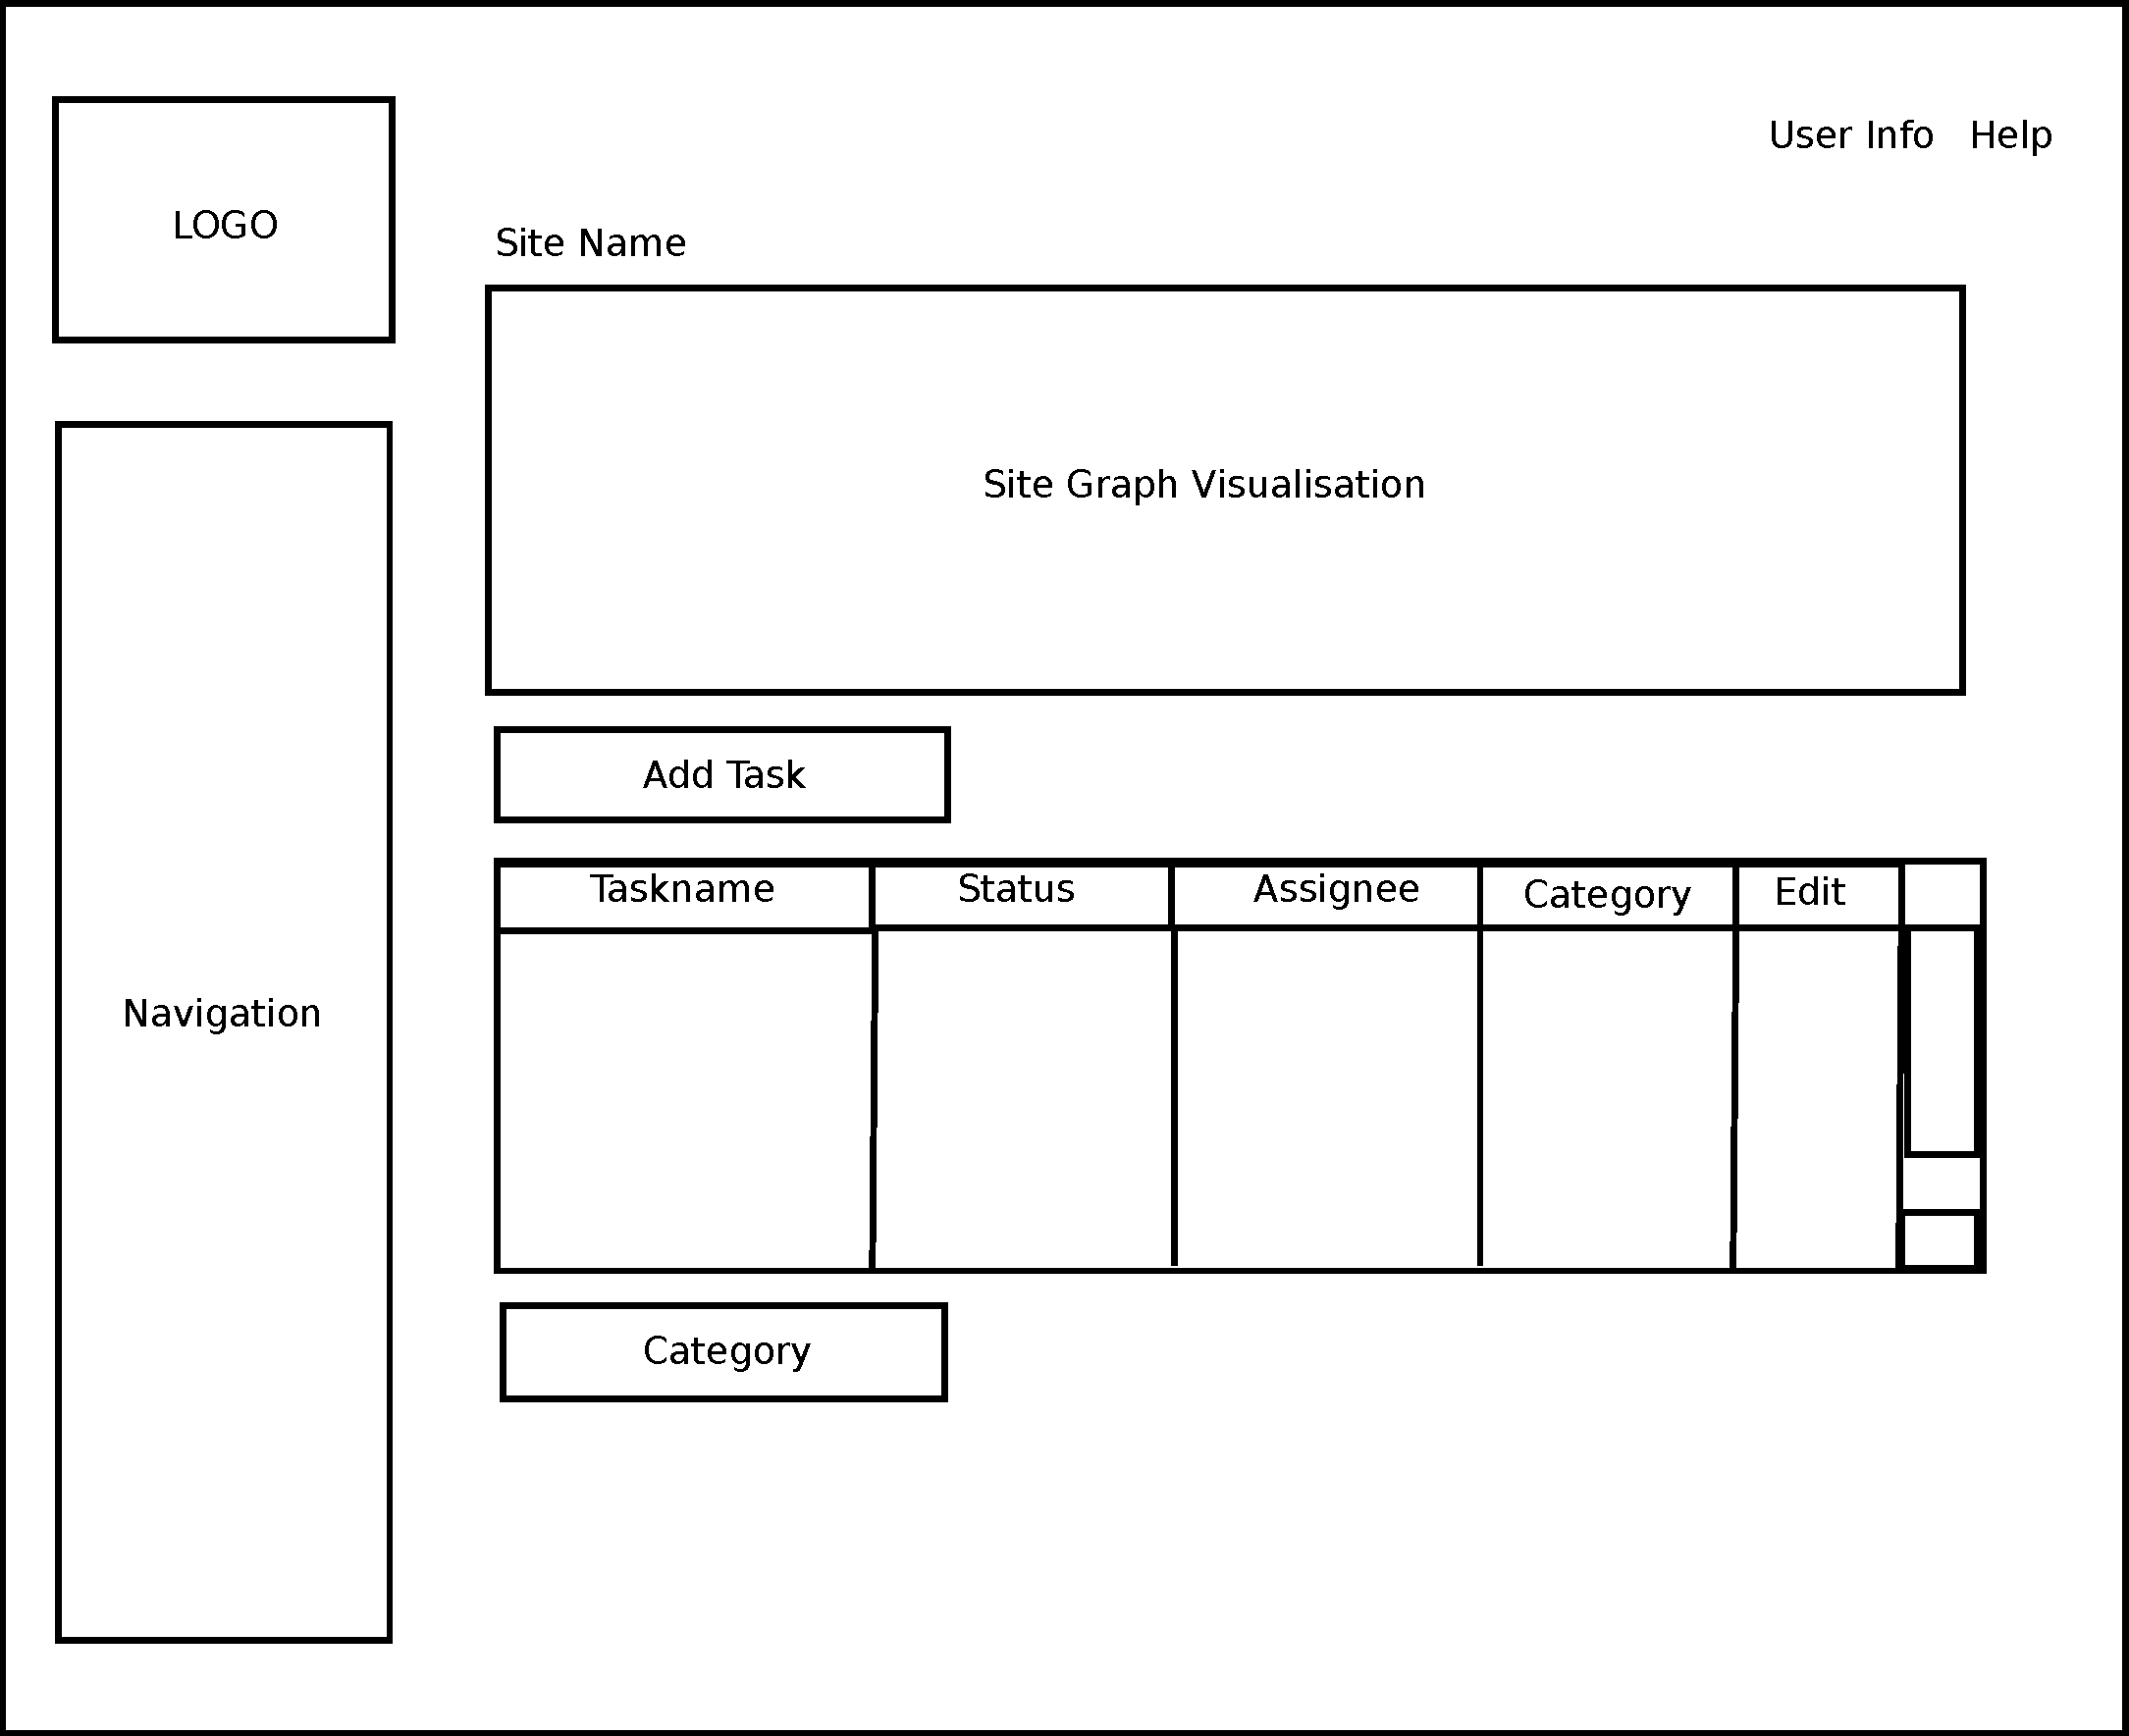
\includegraphics[scale=0.25]{figures/site.pdf}
    \end{center}
    \caption{Site screen developed during the PICTIVE session}
    \label{pictive_site}
\end{minipage}
\hspace{0.5cm}
\begin{minipage}[b]{0.48\textwidth}
    \begin{center}
        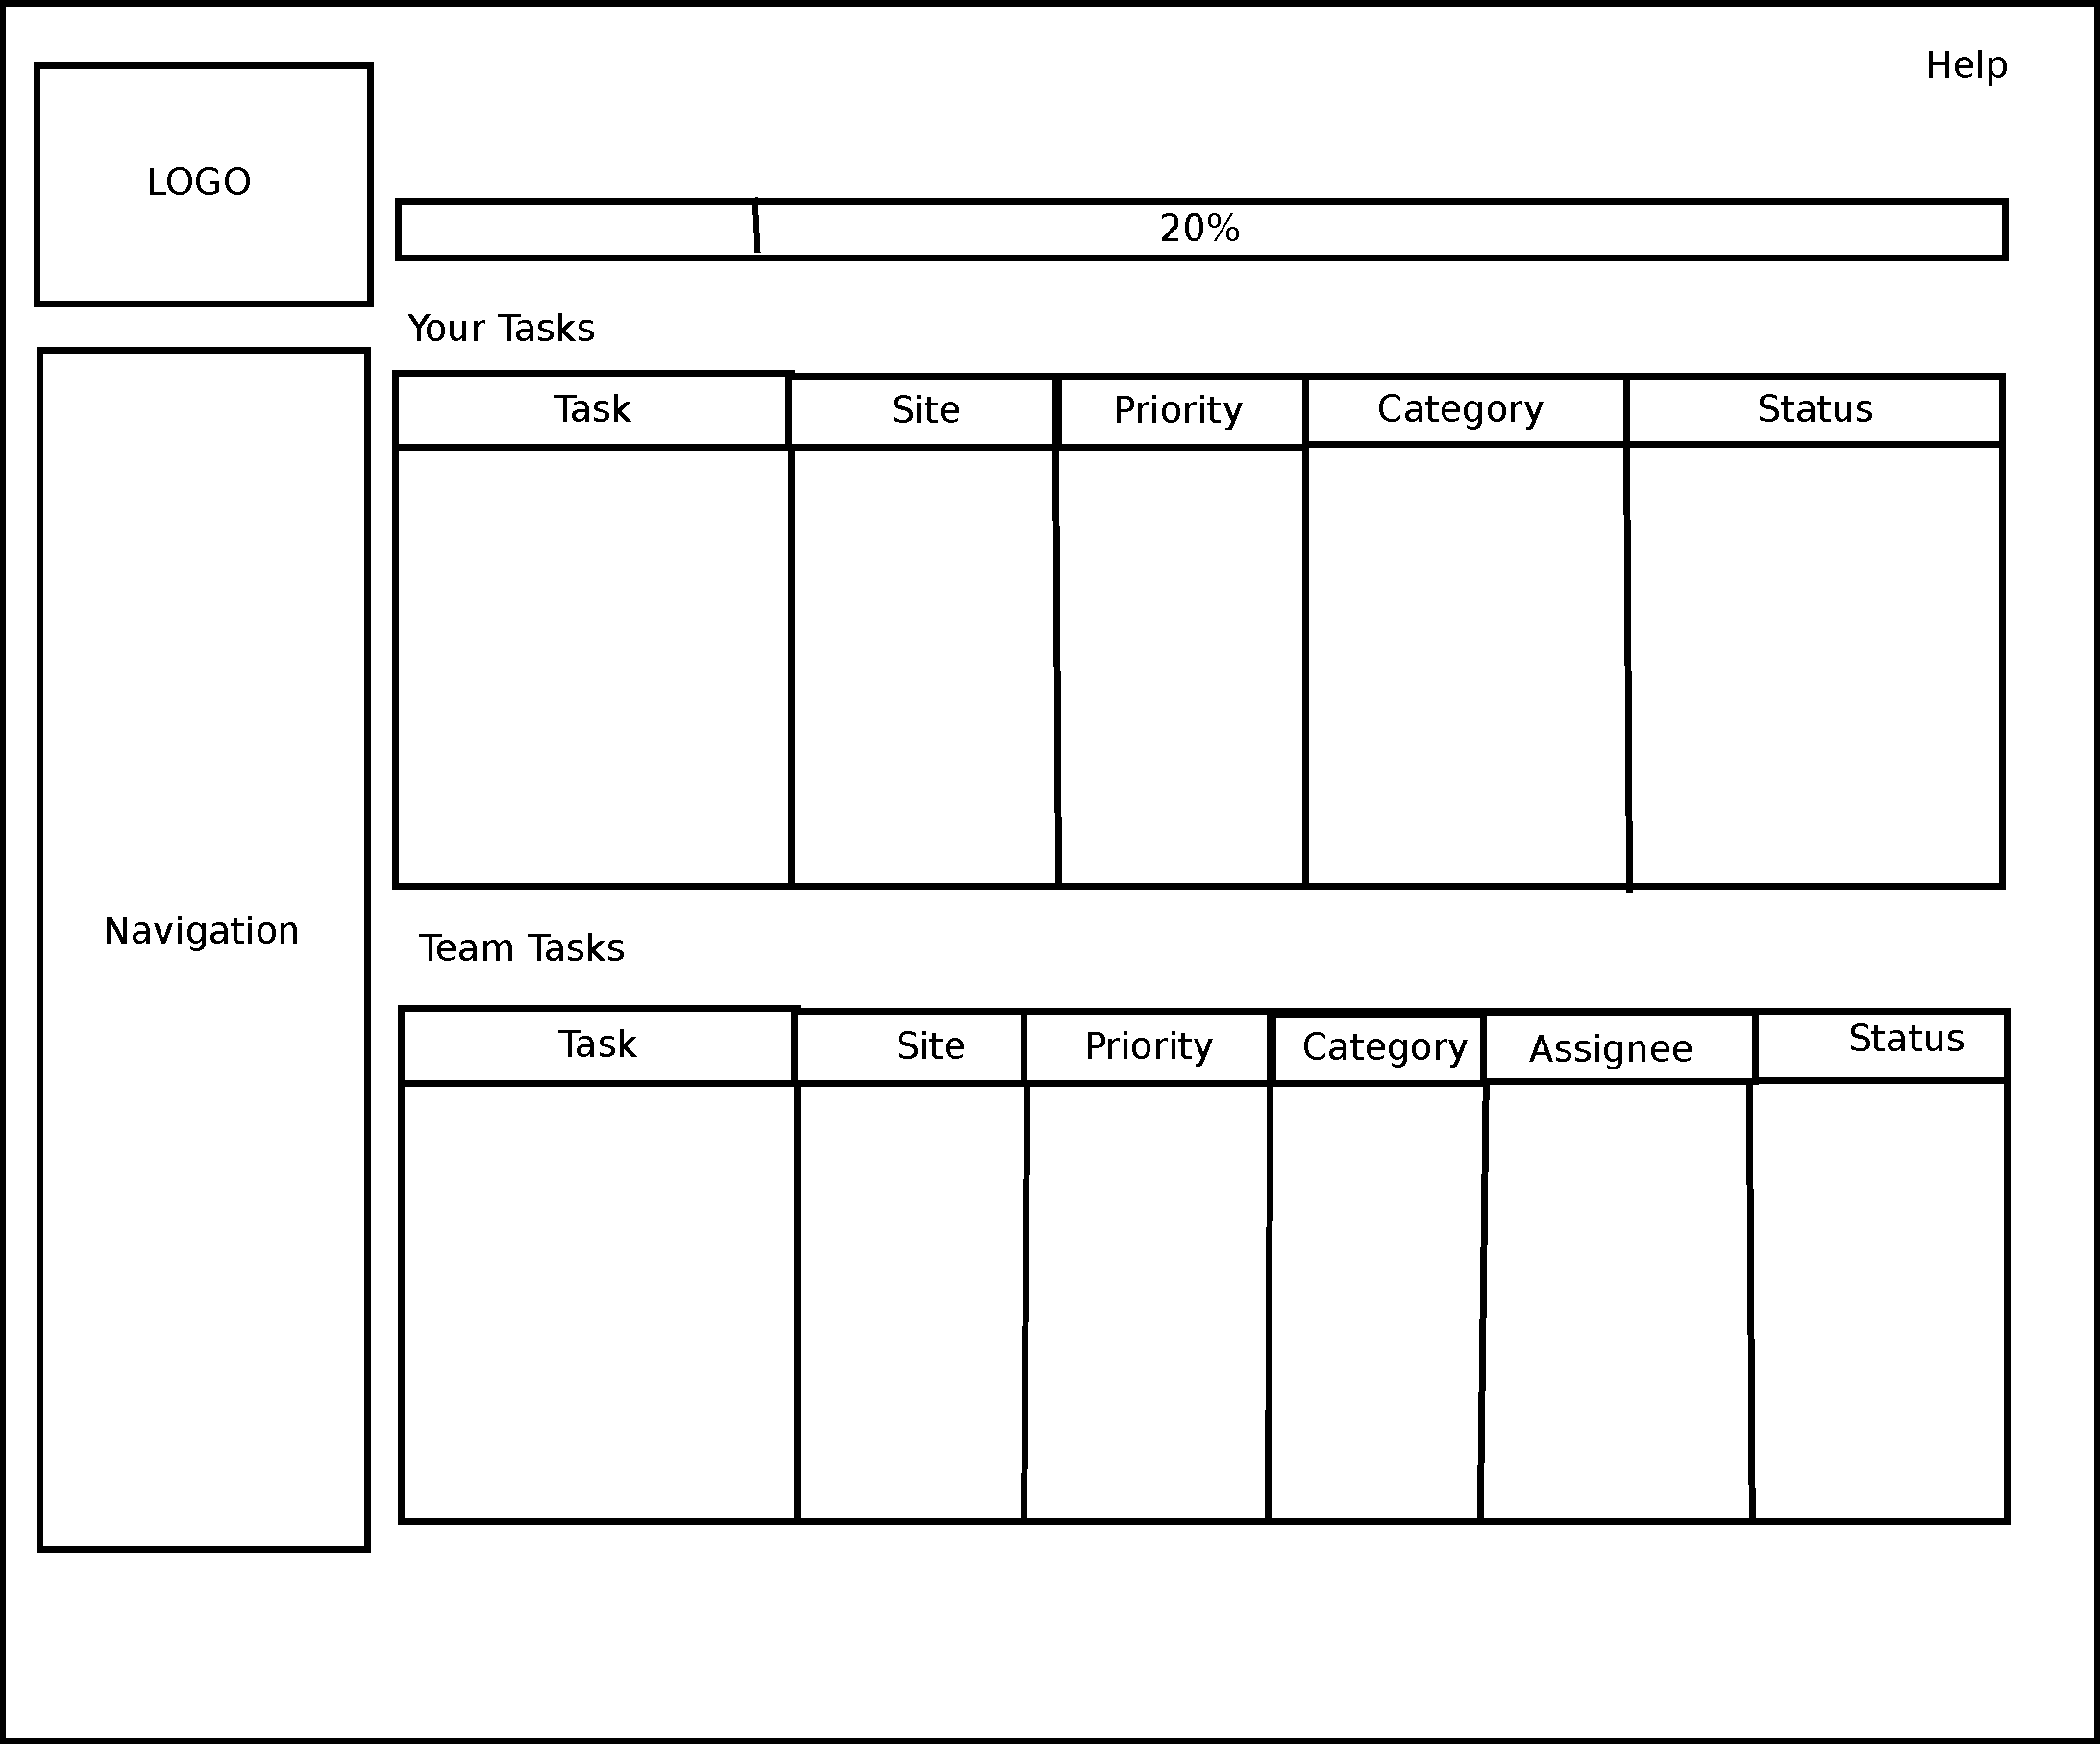
\includegraphics[scale=0.23]{figures/task_list.pdf}
    \end{center}
    \caption{Task Overview screen developed during the PICTIVE session}
    \label{pictive_tasks}
\end{minipage}
\end{figure}

\begin{figure}[!h]
    \begin{center}
        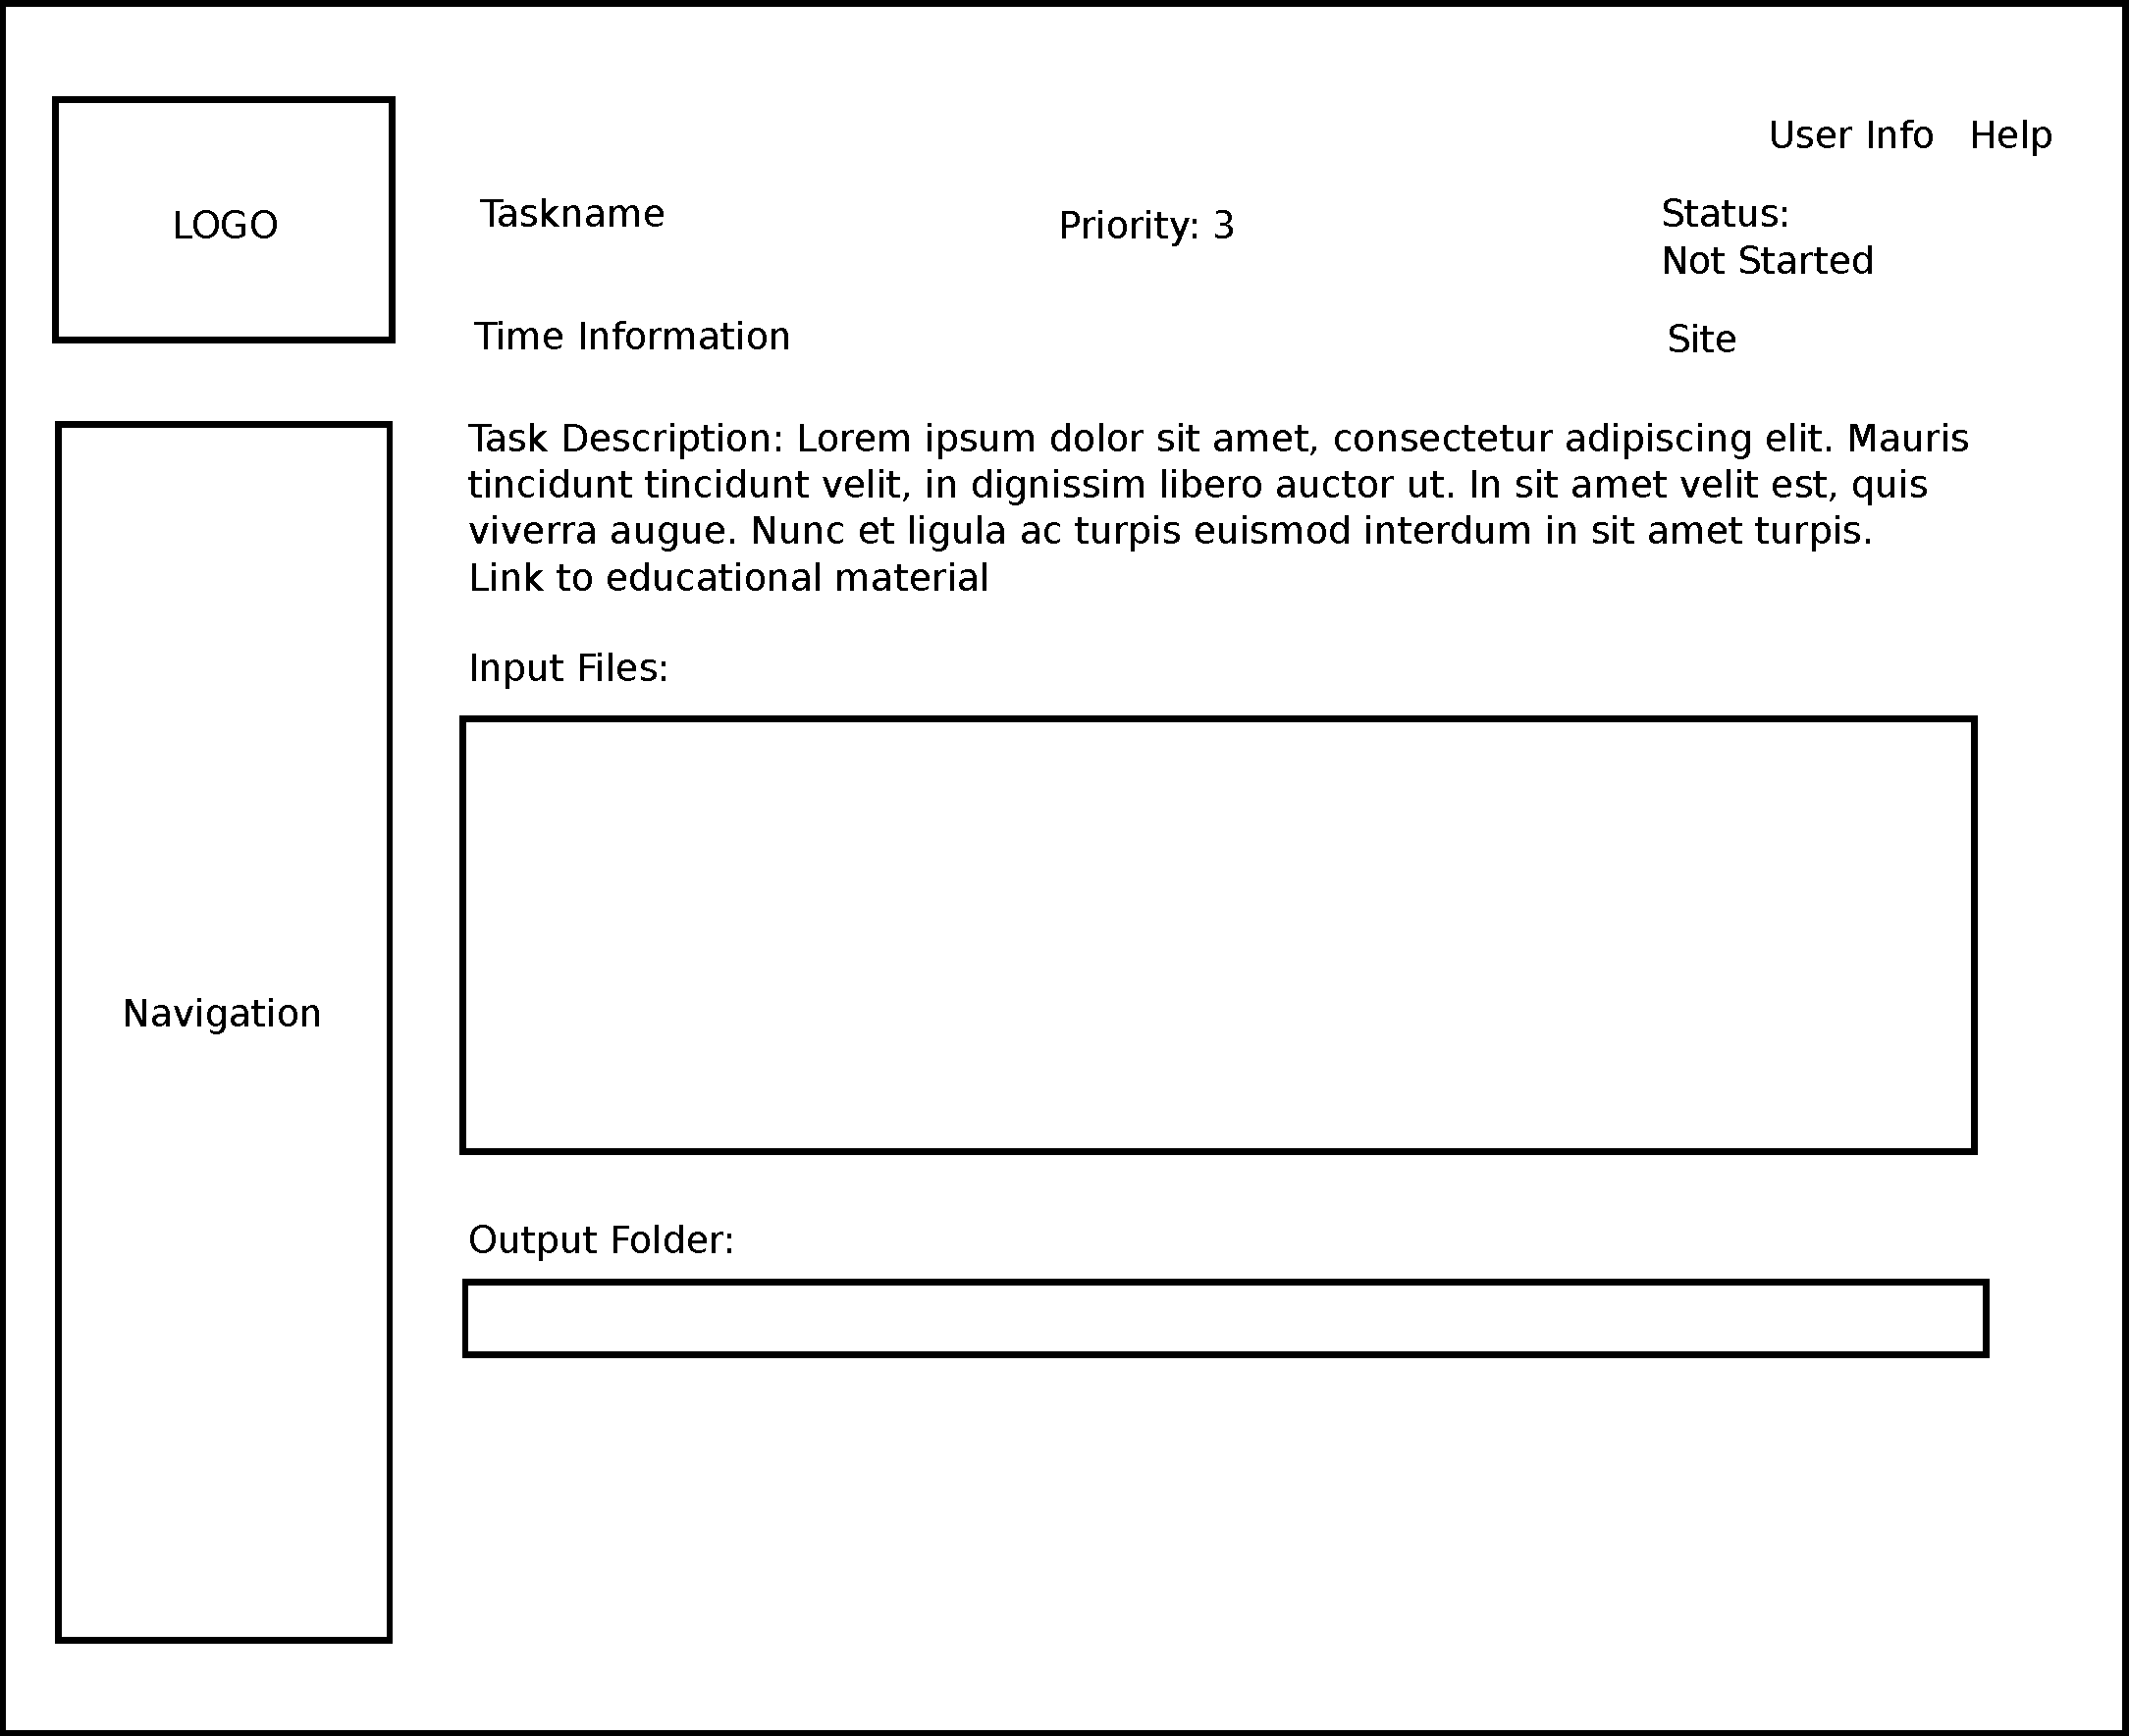
\includegraphics[scale=0.25]{figures/task_overview.pdf}
    \end{center}
    \caption{Task Control screen developed during the PICTIVE session}
    \label{pictive_task}
\end{figure}

\subsubsection{Database Schema\label{db_schema}}
The system needs to manage a large amout of data, this requires
a database that will control all the information required for the
workflow system. to funtion. The primary tables required for this is
\begin{inparaenum}[(i)]
\item Sites;
\item Jobs;
\item Hosts;
\item Files; and
\item Tasks.
\end{inparaenum}

\noindent Each of these tables are described below:
\newpage

\begin{wrapfigure}{l}{7cm}
\begin{tabular}{l|l}
    \multicolumn{2}{c}{Site} \\
    \hline
    Name        & Type \\
    \hline
    Id          & VARCHAR(30) PK \\
    Name        & STRING \\
    Folder Name & STRING \\
    Active      & BOOLEAN \\
\end{tabular}
\caption{Site Schema}
\end{wrapfigure}
\noindent\textbf{Site:}
This table stores the root information for the various sites that
the project is working on. The ``Id'' field is used to for short
\emph{URLs}, while ``Name'' is used for display puposes. ``Folder Name''
provides the root folder that the site data will be stored in. This
allows for consistancy between the repository and the client workstations.
As soon as a site is completed it will also have the option of being marked
inactive. This will prevent the clutter of old sites that no longer require
workflow to be managed.
\\
\begin{wrapfigure}{l}{7cm}
\begin{tabular}{l|l}
    \multicolumn{2}{c}{Job} \\
    \hline
    Name        & Type \\
    \hline
    Id          & AUTOINT PK \\
    Name        & STRING \\
    Type        & CHOICE \\
    Script      & PATH \\
    Description & TEXTFIELD \\
\end{tabular}
\caption{Job Schema}
\end{wrapfigure}

\noindent\textbf{Job:} This table was created to help tasks be more reusable.
The purpose of a given task will be determined by the \emph{Job} that the task
is linked to. This table supports three main type of jobs, namely:
\begin{inparaenum}[(i)] \item User Jobs; \item Server Job: one-to-one; and \item
Server Job many-to-one.\end{inparaenum} This is represented by the type field.
For server tasks the \emph{Script} field is set to a path that contains the
server side script that will execute on the input files defined within a \emph{task}.
For one-to-one tasks  the script is executed once per input file, while it
is executed only once for many-to-one jobs. Information about the job is stored
in the \emph{description} field. The rest of the fields are used to facilitate
naming and queries.
\\
\begin{wrapfigure}{l}{8cm}
\begin{tabular}{l|l}
    \multicolumn{2}{c}{Host} \\
    \hline
    Name        & Type \\
    \hline
    User        & FOREIGNKEY(User)  \\
    Host Name   & STRING  \\
    Root Directory & PATH \\
    Primary      & BOOLEAN \\
\end{tabular}
\caption{Host Schema}
\end{wrapfigure}

\noindent\textbf{Host:} This table manages the control to a user's workstation.
The \emph{user} field points to the user attached to the particular host. While the
\emph{hostname} contians the connection string that connects to the users workstation.
Since every user is likely to have a different folder structure on their workstations,
a \emph{root directory} field was added to indicate a path on the workstation that
will be used as the root folder for the sites. It is very likely that a user could
have more than one workstation, therefore an \emph{primary} field was added to indicate
which host would be the default for that user.
\\

\begin{wrapfigure}{l}{7cm}
\begin{tabular}{l|l}
    \multicolumn{2}{c}{File} \\
    \hline
    Name        & Type \\
    \hline
    Filename    & PATH  \\
    Site        & FOREIGNKEY(SITE)  \\
\end{tabular}
\caption{File Schema}
\end{wrapfigure}
\noindent\textbf{File:} This is a very basic table. Each file will have a database entry
this will add the ability of quick file lookups and aid in maintaining files between the
repository and the workstations. Each entry wil have a \emph{filename} this will store
a relative path from the site root to the file name. By only storing the relative path
we are able to access the file, without making assumptions on where the root directory
is. The second field, links a file to the site that it belongs to.
\\

\noindent \textbf{Task:} This controls the how the workflow is put together in the system.
Each task is defined as an independent actitity that can be executed by the server or
by a user. Each task task has a list of dependencies that need to be satisfied in order
for the task to be executed. When a task is complete its successors are then checked,
and run if all the dependencies are met. In order to ensure that this can be done efficiently
both the predecessors and the successors are stored in the table. The \emph{Id} field is
used for task identification in urls. Each task also has time information, the execution
time of a

\begin{wrapfigure}{l}{7cm}
\begin{tabular}{l|l}
    \multicolumn{2}{c}{Task} \\
    \hline
    Name        & Type \\
    \hline
    Id              & AUTOINT PK  \\
    Priority        & INTEGER  \\
    Started         & DATETIME \\
    Ended           & DATETIME \\
    Log             & TEXTFIELD \\
    Site            & FK(Site) \\
    Job             & FK(Job) \\
    Assignee        & FK(User) \\
    Input Files     & MTM(File) \\
    OuputFolder     & PATH \\
    Predecessors    & MTM(Task) \\
    Successors      & MTM(Task) \\
    Job Status      & CHOICE FIELD \\
\end{tabular}
\caption{Task Schema}
\end{wrapfigure}
\noindent task can be calculated by subtracting the start time from the end time. Each
task is based on a \emph{Job} this allows jobs to be reused in various tasks making the
system easier to use. A task is explicitly assigned to a user, for automatics tasks a
dummy user named ``server'' is used to ensure database consistancy. The inputfiles of
a task is defined in a ``Many-to-Many''\footnote{MTM refers to Many-To-Many Field}
field, this enables the system to only transfer
required files to workstations as well as running the script on appropriate data. When
a task is executing the system expects the output files to be placed in the output folder
field, this allows the sytem to manage the file dependencies of the successor tasks.

Along with the system being failure tolerant it also needs to be able to determine what
has happend when a failure has occured. For this reason a \emph{Log} field was added this
field stored all the activity that a task performs. This includes the transfer logs as
well as any output generated during the execution of the server scripts. Tasks are also
stateful; this state is represented by the \emph{Job Status} field. The possible states
for a task are:
\begin{inparaenum}[(i)]
\item NOT DONE;
\item TRANSFERRING;
\item IN PROGRESS;
\item TRANSFERING BACK;
\item VALIDATION REQUIRED;
\item DONE; and
\item FAILED.
\end{inparaenum}

\subsubsection{Features}
All these components were put together to support the required features of the system. Below
are a list of features that were implement during this design iteration.
\begin{description}
    \item[File Transfer] \hfill \\
        User tasks are able to transfer files to the user workstations, from the input
        file list. As soon as a task is user task is triggered the file list is retrieved
        from the task entry. The server then connects to to the host and copies over all
        the required files. Since a user can have more than one host this transfer can also
        be manually triggered by the user. When a task is then completed the server will
        again initialise the file transfer but in the opposite direction. All files that
        are present in the \emph{Output Directory}. In order to support switching of workstations
        this process can also be triggered at any stage, before the task is completed.
        Extra functionality is also added to download all the files in the output directory
        located on the server.
    \item[Task Automation] \hfill \\
        The systems abilty to facilitate workflows is entirely dependent on its ability
        to automate tasks. This is done by adding a control system within the server
        that works out which tasks have no unmet dependencies. As soon as these tasks
        have been determined an asynchronis task is launched to run the task. Depending on
        the type of job either files are transfered or a script is run. When a task is
        completed, either by verification or the script finishing, the task is finalised.
        This process involves adding all the generated files to the database, updating the
        input files of the successors. If all the dependencies of a successor is met that
        task is then started. When a task fails however a user is able to make the required
        changes and restart the process.
    \item[Logging] \hfill \\
        Logging is added to help with identifying and controlling task failures. Within
        the automisation framework all events happening with the task is added to an
        append only log field. This includes the transfer logs for user tasks, and both
        \emph{stdout} and \emph{stderr}.
    \item[Site Visualisation] \hfill \\
        The tasks for a site can be represented as a \emph{Directed-Acyclic-Graph}. To
        make the system a bit more user friendly, the tasks will be represented as
        graph within the interface. This is done by calculating the a the graph of
        the sites and then applying a layout algorithm to it. For the purposes of this
        viualisation a spring layout is used. The nodes are then joined by edges. A
        summary of each task is displayed on the node.
    \item[Site Setup] \hfill \\
        Priveledged users should be able to compose workfloews with relative ease. Options
        are added to allow users to create new Jobs and task. Once a task is added dependencies
        can then be added in a visual way on the visualisation. Workflows between sites are very similar
        creating a new workflow for each site would be very time consuming. An additional
        feature is added that copies over the structure of an existing site, and then
        just requires the files to be chosen.
\end{description}
\subsection{Implementation}
The system was implemented using the \emph{Django framework}. This was done in 3 parts:
\begin{inparaenum}
\item database setup
\item workflow framework; and
\item user interface.
\end{inparaenum}

The \emph{database} was setup using the model subsystem in \emph{Django}, from the chosen schema.
This is a system that uses a defines the database using python, this allows the schema
to be implemented without needing to worry about the database system being used. For the
purpose of this iteration \emph{SQLite}\footnote{SQLite: www.sqlite.org} was used to
support the database. This can however easily be changed to a more robust system as the demand
on the system grows. User data was implemented using the authentication module in Django. This
module manages users and permissions on the system. As the schema was discussed in Section~\ref{db_schema}
it will not be discussed further.

\subsubsection{Workflow Framework}
The underlying workflow system is implemented using \emph{Python}\footnote{Python: www.python.org}, within
the Django framework. Tasks are executed asynchronously. Each job type is handled separately.
\begin{description}
\item[Server Job - One to One] \hfill \\
    This job type executed a given script on all the input files. The system generates a list of
    absolute paths and executes the script given two parameters, the input file, and the output
    directory. This is done for all the files input files of the task.
\item[Server Job - Many to One] \hfill \\
    This job type executes nearly identically to the \emph{One to One} task, however instead
    of the script being run run multiple times, it is run once, here however all input files
    are passed in as arguments, along with the output directory. Both server jobs can use
    any script or applications available on the system. With applications where the parameter
    structure does not match the required utility wrapper scripts can be used.
\item[User Job] \hfill \\
    This type of job is split into multiple parts. Since there is a distinct separation between
    the server and the execution of type of task, the goal is to ensure the effective communication
    between workstations and servers. The goal is to be able to transfer large amounts of files
    with minimal redundancy. For this reason \emph{rsync}\footnote{Rsync Incremental file
    transfer: rsync.samba.org} is used. This only transfers files that have not been been transfered
    yet, as such redundancy is greatly reduced, and enables efficient recovery in case of network failure.

    Figure~\ref{user_task_impl2} shows the components used to execute a user task. Each of these components
    are built using an asynchronous object. Note that the transfer components can be used at any point
    during the task's life cycle.
\end{description}
\begin{figure}[!h]
    \begin{center}
        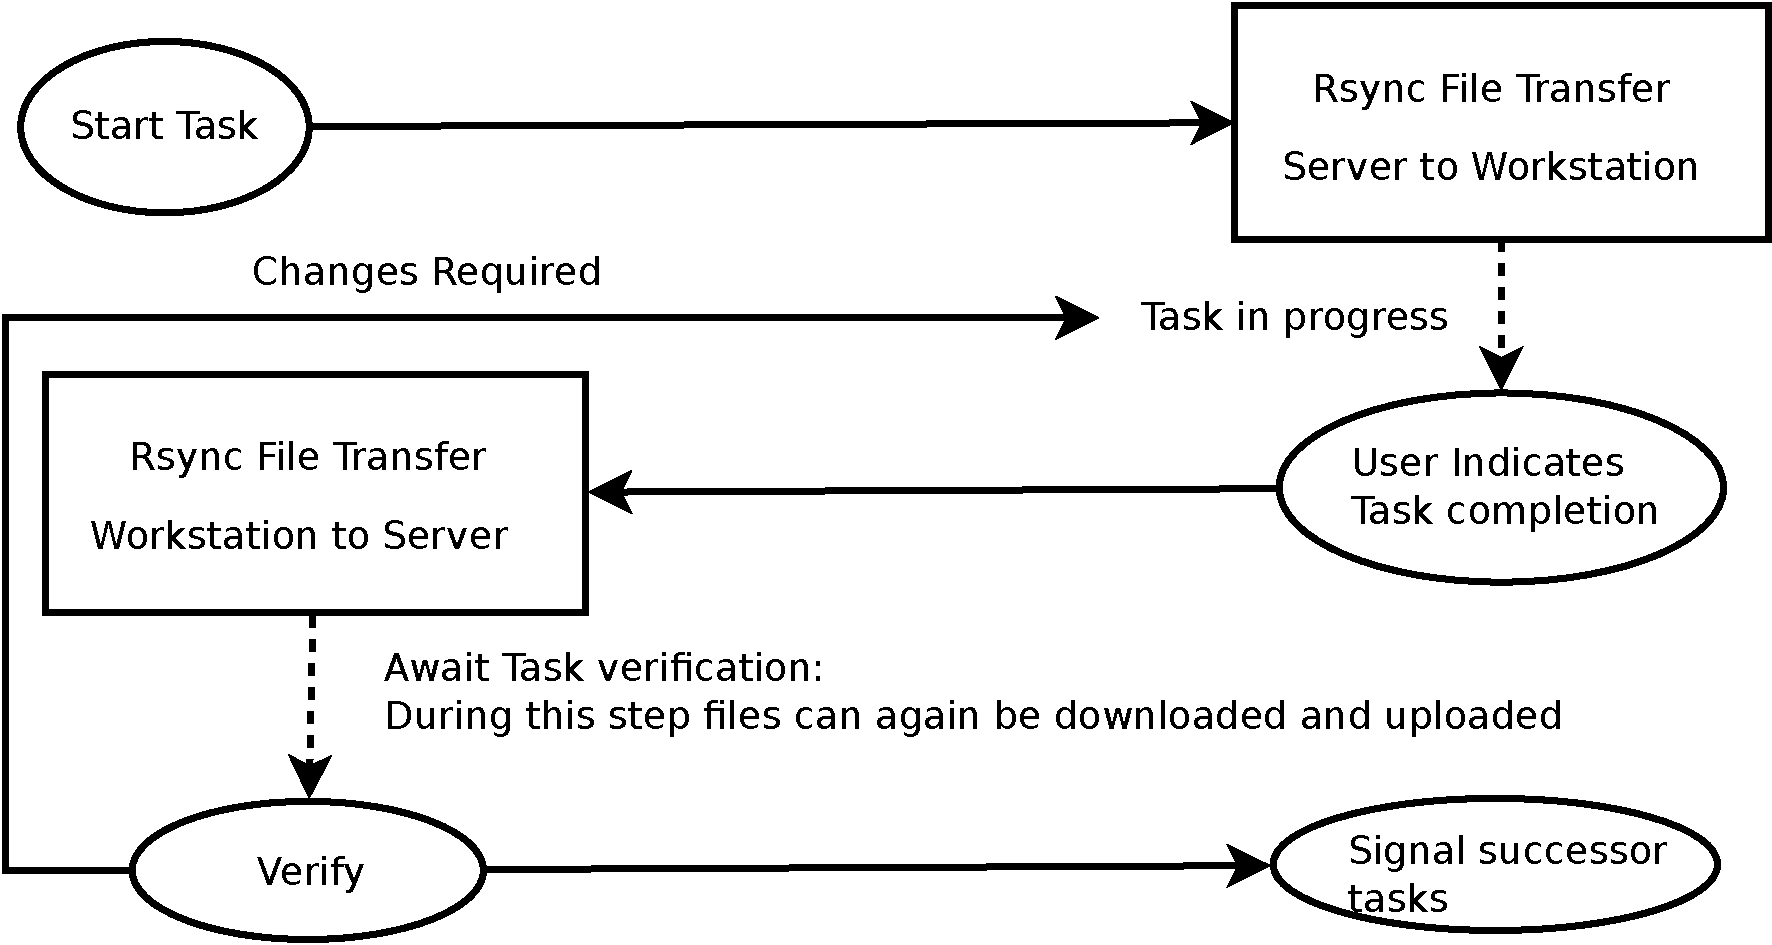
\includegraphics[scale=0.4]{figures/user_impl2.pdf}
    \end{center}
    \caption{Components that support user jobs}
    \label{user_task_impl2}
\end{figure}
    Once a task is finished it passes on to finalisation. All tasks follow this model. It
    is assumed that all the appropriate files are present on the server at this point and
    that the task has completed successfully. At this the output directory is scanned for
    files recursively, new files are indexed and added to the database. The new files are then
    added to the input files of all successor tasks. If all the dependencies of a successor
    task is met the task is then launched.

\subsubsection{User Interface}
The interface was implemented using \emph{HTML} served using the View subsystem in Django.
These views aim to create a usable system. These are based on the designs that were created
during the \emph{PICTIVE} session. Slight alterations were made to the design to support required
functionality that was not considered during the session. The interface comprises out of several
views.
\begin{description}
\item[Task Overview] \hfill \\
    This view has the purpose showing a user which tasks are outstanding. As well as show what is
    happening within the team. This also provides links to the task control page for each task.
    An additional feature that was implemented allows users to filter tasks based on a choice
    of sites.
\item[Task Control] \hfill \\
    This is the view that non-privileged users will be interacting with most often. It provides
    a detailed overview of what is required to be done with the task. Privileged users also
    get a link to edit the task. This page also contains tools to allow users to download
    and upload required files. Once a user is finished with the task at hand he/she can
    simply press on the \emph{Finish Task} button. This triggers the transfer back routine
    and queues the task for verification. Users who are able to verify the task will use the
    same view however the \emph{Finish Task} button is replaced with two buttons that will
    accept or reject the task. Logging information is also made visible to ensure that the
    complete task history is visible.

    This view is also used for server tasks. In this case the emphasis is on failure control.
    With the log visible user can trace the source of the failure and rerun the task as soon
    as it is has been dealt with.

\item[Task Editing] \hfill \\
    During the initial task setup the parameters of a task need to be set. This screen enables
    the user to set the who the task is assigned to, what the input files are, and what the task
    depends on. Note that the dependencies can also be set on in a friendly way on the task interface.
    When something goes wrong with a tasks privileged users are also able to edit these setting
    when the workflow is already active. The workflow should be able to dynamically adapt in this case.
\item[Site View] \hfill \\
    This view is dominated by the visualisation of the site. The visualisation was implemented using
    \emph{jsPlumb}\footnote{jsPlumb Graph UI: jsPlumb.org}. This an API based that builds interactive
    graphs. Each node provides and overview of the task. Dependencies are represented with edges
    while the colour of the node indicates the status of task. Red indicates that there is a
    problem with the task, grey indicates that the task has not been run, blue indicates the
    task is in progress and green indicates that the task has been successfully completed. Dependencies
    can be added by dragging an edge from corner to another task.

    Below the visualisation is a list of the tasks in the site. This gives an overview
    similar to the task overview screen. A privileged user can tasks off given jobs
    from here which will then forward to the task editing screen.
    As soon as the tasks in a site has been set up, the workflow can be started from this view.

    The final set of components is there to add/edit jobs and categories in the system. These
    are not specifically linked to a site and as such can be used throughout the system allowing
    for easy reuse.
\end{description}
In addition to \emph{jsPlumb}, \emph{jQuery} and \emph{jQuery UI} is used extensively to build
the client side interface.
\subsection{Evaluation}




\section{Iteration 3\label{iteration3}}


\bibliography{bibliography}{}
\bibliographystyle{apalike}


\end{document}
